

\begin{tikzpicture}[scale=1.1],

\begin{axis}[xlabel=$x$,
ylabel= $\delta$,
height=6cm,
width=10cm,
ymax=11,
ymin=0,
xmin=0,
xmax=6.5,
axis y line=left,
axis x line=bottom,
ytick={1,...,10},
yticklabels={ ,,$f(a)$ ,,},
xtick={1,...,5},
xticklabels={$x_0$,$x_2$,$a$,$x_3$,$x_1$,}
]
  \addplot[dashed] coordinates {(0,1.5) (1,1.5)};
  \addplot[dashed] coordinates {(1,0) (1,1.5)};
  \addplot[dashed] coordinates {(0,2) (2,2)};
  \addplot[dashed] coordinates {(2,0) (2,2)};
  \addplot[blue,dashed] coordinates {(0,3) (3,3)};
  \addplot[blue,dashed] coordinates {(3,0) (3,3)};
  \addplot[dashed] coordinates {(0,5) (4,5)};
  \addplot[dashed] coordinates {(4,0) (4,5)};
  \addplot[dashed] coordinates {(0,9) (5,9)};
  \addplot[dashed] coordinates {(5,0) (5,9)};

    \addplot[black,domain=1:9]  { 2^(\x-2)+1  }node {f};
    


\end{axis}
\end{tikzpicture}



\begin{tikzpicture}[scale=1.1],

\begin{axis}[xlabel=$x$,
ylabel= $\delta$,
height=6cm,
width=5cm,
ymax=3,
ymin=0,
xmin=0,
xmax=2,
axis y line=left,
axis x line=bottom,
ytick={1,...,10},
yticklabels={ 1,2},
xtick={1,...,5},
xticklabels={$1$}
]
    \addplot[black,domain=0:1]{x+1}node[above, sloped, pos = 0.3] {g};
    \addplot[black,domain=1:2]{x+1}node[above, sloped, pos = 0.65] {f};
    \draw [blue,  -stealth    ] (3,1) -- (1.1,2) node [right] {Lücke};
    \addplot[mark=*,fill=white] coordinates {(1,2)};

\end{axis}
\end{tikzpicture}


\begin{tikzpicture}[scale=1.1],

\begin{axis}[xlabel=$x$,
ylabel= $y$,
height=6cm,
width=5cm,
ymax=3,
ymin=-3,
xmin=-3,
xmax=3,
axis y line=center,
axis x line=center,
]
\addplot[domain= -3:-0.01] {1/x};
\addplot[domain= 0.01:3] {1/x};


\end{axis}
\end{tikzpicture}




\begin{tikzpicture}[scale=1.1],

\begin{axis}[xlabel=$x$,
ylabel= $y$,
height=6cm,
width=5cm,
ymax=3,
ymin=-3,
xmin=-3,
xmax=3,
axis y line=center,
axis x line=center,
]
\addplot[domain= -3:-0.01] {1/x};
\addplot[domain= 0.01:3] {1};


\end{axis}
\end{tikzpicture}

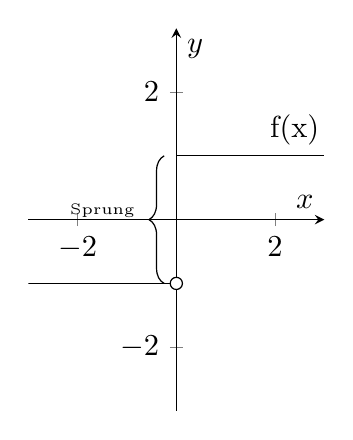
\begin{tikzpicture}[scale=1.1],

\begin{axis}[xlabel=$x$,
ylabel= $y$,
height=6cm,
width=5cm,
ymax=3,
ymin=-3,
xmin=-3,
xmax=3,
axis y line=center,
axis x line=center,
]
\addplot[domain= -3:0] {-1};
\addplot[domain= 0:3] {1} node[above ,pos=0.8] {f(x)};
\addplot[mark=*,fill=white] coordinates {(0,-1)};
  \draw [decorate, decoration={brace,amplitude=5pt,raise=4pt,mirror}] (0,1) -- (0,-1) 
node [midway, xshift=-0.5mm, yshift=1mm,auto, swap, outer sep=9pt,font=\tiny]{Sprung};
\end{axis}
\end{tikzpicture}


\begin{tikzpicture}[scale=1.1],

\begin{axis}[xlabel=$x$,
ylabel= $y$,
height=6cm,
width=5cm,
ymax=3,
ymin=-3,
xmin=-3,
xmax=3,
axis y line=center,
axis x line=center,
]
\addplot[domain= -3:-0.01] {1/x};
\addplot[domain= 0.01:3] {1/x};


\end{axis}
\end{tikzpicture}


\begin{tikzpicture}[scale=1],

\begin{axis}[xlabel=$x$,
ylabel= $y$,
height=12cm,
width=17.5cm,
ymax=5,
ymin=-3,
xmin=-3,
xmax=3,
axis y line=center,
axis x line=center,
]
\addplot[domain= -3:-0.01] {1/x};
\addplot[domain= 0.01:3] {1/x};
\draw [red,  -stealth    ] (-0.5,0.7) -- (-0.1,0.1) node [left,pos=0] {kein intervall im  Definition Bereich};
\addplot[mark=*,fill=white] coordinates {(0,0)};
\addplot[ very thick,mark options={solid},blue,domain= 0.8:2.3] {1/x};
\addplot[ very thick,mark options={solid},blue,domain= 0.8:2.3] {0};
\draw [blue,  -stealth    ] (0.5,-2) -- (1.2,-0.6) node [below,pos=0] { intervall };

\end{axis}
\end{tikzpicture}



\begin{tikzpicture}[scale=1.2],

\begin{axis}[
height=6cm,
width=10cm,
ymax=11,
ymin=0,
xmin=0,
xmax=6.5,
axis y line=left,
axis x line=bottom,
ytick={1,...,10},
yticklabels={ ,$f(a)-\epsilon$ ,,,,$f(x)$,,,$f(a)+\epsilon$},
xtick={1,...,5},
xticklabels={,,$a-\delta$,$a$,$a+\delta$}
]
\addplot[dashed] coordinates {(0,2) (2,2)};
\addplot[dashed] coordinates {(2,0) (2,2)};
\addplot[blue,dashed] coordinates {(0,3) (3,3)};
\addplot[blue,dashed] coordinates {(3,0) (3,3)};
\addplot[dashed] coordinates {(0,5) (4,5)};
\addplot[dashed] coordinates {(4,0) (4,5)};
\addplot[blue,dashed] coordinates {(0,9) (5,9)};
\addplot[blue,dashed] coordinates {(5,0) (5,9)};

\addplot[black,domain=1:9,name path=A]  { 2^(\x-2)+1  } node at (5.5, 8.5) {f};
\addplot[very thick,blue,name path=B,domain= 3:5] {0};
\addplot[blue,very thick] coordinates {(0,3) (0,9)};
\addplot[gray, pattern=north west lines] fill between[of=A and B, soft clip={domain=3:5}];
\legend{$qeg \; \epsilon$, $gce \; \delta$}



\end{axis}
\end{tikzpicture}


